% FLAMINGO galaxy-matter cross spectrum: measurement and the scale dependence of the galaxy bias.
% Build with assets/build_note.sh of the summary-notes skill.
\documentclass[11pt]{article}

\usepackage[margin=1in]{geometry}
\usepackage{amsmath}
\usepackage{amssymb}
\usepackage{graphicx}
\usepackage{booktabs}
\usepackage{xcolor}
\usepackage[font=small,labelfont=bf,labelsep=period]{caption}
\usepackage[hidelinks]{hyperref}

\newcommand{\hMpc}{\,h\,{\rm Mpc}^{-1}}
\newcommand{\Pgm}{P_{\rm gm}}
\newcommand{\Pgg}{P_{\rm gg}}
\newcommand{\Pdm}{P_{\rm dm}}
\newcommand{\Pm}{P_{\rm m}}
\newcommand{\bgm}{b_{\rm gm}}
\newcommand{\bgg}{b_{\rm gg}}

% =====================================================================
% Numbers
% =====================================================================
\newif\ifnumbersfinal
\numbersfinaltrue
\newcommand{\refresh}[1]{\ifnumbersfinal#1\else\textcolor{red}{#1}\fi}
% Part 1: results (plots/numbers.json, written by plots/make_figure_data.py)
% large-scale bias b1 from P_gm and from P_gg, z = 1.5, 2, 3
\newcommand{\bOneA}{\refresh{1.874}}
\newcommand{\bOneB}{\refresh{2.216}}
\newcommand{\bOneC}{\refresh{3.215}}
\newcommand{\bOneGgA}{\refresh{1.874}}
\newcommand{\bOneGgB}{\refresh{2.217}}
\newcommand{\bOneGgC}{\refresh{3.237}}
% k_max = K0/D(z) of the w cut (K0 = 0.2) and the gamma_t cut (K0 = 0.5) [h/Mpc]
\newcommand{\kwA}{0.40}
\newcommand{\kwB}{0.48}
\newcommand{\kwC}{0.63}
\newcommand{\kgA}{1.0}
\newcommand{\kgB}{1.2}
\newcommand{\kgC}{1.6}
% b_gg/b1 at the w k_max and b_gm/b1 at the gamma_t k_max, in per cent above linear
\newcommand{\wA}{\refresh{8}}
\newcommand{\wB}{\refresh{18}}
\newcommand{\wC}{\refresh{43}}
\newcommand{\gA}{\refresh{19}}
\newcommand{\gB}{\refresh{41}}
\newcommand{\gC}{\refresh{92}}
% r (Poisson-subtracted) at k = 0.3 and raw r at 0.3, 1 (no subtraction)
\newcommand{\rA}{\refresh{1.000}}
\newcommand{\rB}{\refresh{0.994}}
\newcommand{\rC}{\refresh{0.952}}
\newcommand{\rFiveLo}{\refresh{1.29}}
\newcommand{\rFiveHi}{\refresh{1.46}}
\newcommand{\rRawOneLo}{\refresh{0.76}}
\newcommand{\rRawOneHi}{\refresh{0.89}}
% the whole Poisson term at the w k_max, as a fraction of b_gg [per cent] (numbers.json, shot_w)
\newcommand{\ShotWA}{\refresh{5}}
\newcommand{\ShotWB}{\refresh{7}}
\newcommand{\ShotWC}{\refresh{15}}
% checks
\newcommand{\FoldA}{0.3}     % max |b_gm(fold 4)/b_gm(fold 1) - 1| at k = 0.3 to 1, per cent
\newcommand{\FoldB}{0.5}
\newcommand{\FoldC}{1.7}
\newcommand{\OldShape}{1.2}  % max difference of b(k)/b(0.04 to 0.1) from the earlier P_hh-only table, per cent
\newcommand{\OldNorm}{1.5}   % shift of the low-k b from the earlier table, per cent
% Part 2: inputs and run facts
\newcommand{\NdmTot}{46{,}656{,}000{,}000}
\newcommand{\NgA}{4{,}808{,}380}
\newcommand{\NgB}{3{,}661{,}123}
\newcommand{\NgC}{1{,}613{,}396}
\newcommand{\TA}{6.9}        % stream wall time [h], logs/matter_cross.log
\newcommand{\TB}{6.7}
\newcommand{\TC}{5.5}
\newcommand{\Rate}{2.0}      % 10^6 rows/s

\title{The galaxy-matter cross spectrum of FLAMINGO\\ and the scale dependence of the galaxy bias}
\author{Yijie Zhu}
\date{November 21, 2026}

\begin{document}
\maketitle

\section{Summary}

\textbf{Question.} How far does linear galaxy bias hold for the galaxy-galaxy
lensing ($\gamma_t$) and clustering ($w$) parts of 3x2pt, at the redshifts
where the earlier estimate from the galaxy auto spectrum alone found it
failing ($z \ge 1.5$)? $\gamma_t$ sees the galaxy-matter cross spectrum $\Pgm$,
which no FLAMINGO data product holds, so it was measured here.

\textbf{Answer.} On large scales linear bias holds: the biases from $\Pgm$ and
from $\Pgg$ agree to 0.1\% at $z = 1.5$ and 2 and to 0.7\% at $z = 3$, and the
cross-correlation coefficient is $r = 1$. At the 3x2pt baseline cuts the bias
has grown well above linear (Figure~\ref{fig:bias_k}): at the $w$ cut
($K_0 = 0.2$) $\bgg$ is \wA, \wB\ and \wC\% above its large-scale value at
$z = 1.5$, 2 and 3, and at the $\gamma_t$ cut ($K_0 = 0.5$) $\bgm$ is \gA, \gB\
and \gC\% above. Up to $k \approx 0.5\hMpc$ the two biases agree to 1.5\% at
$z \le 2$, so $\Pgm = \bgg \Pm$ is a good approximation there; at $z = 3$
$r$ falls to \rC\ by $k = 0.3\hMpc$.

\textbf{Method.} Every dark-matter particle of the L1\_m8 snapshots at
$z = 3$, 2 and 1.5 ($3600^3$ each) was streamed from the COSMA data server onto
the grids of the galaxy field, so $\Pdm$, $\Pgm$ and $\Pgg$ share one grid,
window and set of modes. The scale-dependent biases are ratios of these
spectra, in which the window, the aliasing and most of the sample variance
cancel.

\textbf{Limits.} The galaxies are the IA shape sample ($10 < \log M_* < 11.1$
to 11.35), not Roman's lenses, though their biases are close. The matter
field is dark matter only, moved to the total matter with the SWIFT spectra
(a 1 to 2\% factor). $\bgg$ depends on the galaxy noise model (the Poisson term is \ShotWA\ to
\ShotWC\% of $\bgg$ at the $w$ cuts, and above $k \approx 1\hMpc$ the noise
is sub-Poisson, Figure~\ref{fig:cross_r}); $\bgm$ does not.

\section{Fiducial setup}

\begin{itemize}
\item \textbf{Simulation.} FLAMINGO L1\_m8 (hydrodynamical, $681\,h^{-1}$Mpc box,
  $3600^3$ dark-matter particles), D3A cosmology: $\Omega_{\rm m} = 0.306$,
  $\Omega_{\rm b} = 0.0486$, $h = 0.681$, $\sum m_\nu = 0.06$\,eV.
\item \textbf{Snapshots.} 48 ($z = 1.5$), 38 ($z = 2$), 18 ($z = 3$). The
  $z = 1$ snapshot was not streamed: there the bias from $\Pgg$ is linear to
  4\% out to $k = 1\hMpc$.
\item \textbf{Galaxies.} The IA shape sample of the FLAMINGO IA pipeline:
  subhalos with at least 100 star particles and
  $0.681 < M_*/(10^{10}\,h^{-1}M_\odot) < 8.57$, 11.57, 15.25 at
  $z = 1.5$, 2, 3, centrals and satellites ($N_{\rm g} = \NgA$, \NgB,
  \NgC).
\item \textbf{Grids.} Nearest-grid-point assignment, the box folded 1, 4 and 16
  times ($n_g = 1024$, 1024, 512); fold $f$ is used for
  $\tfrac14 k_{\rm Nyq}(f/4) < k \le \tfrac14 k_{\rm Nyq}(f)$. 30 logarithmic
  bins from 0.003 to $20\hMpc$, as for the IA spectra.
\item \textbf{Cuts.} The 3x2pt baseline keeps scales with
  $k < K_0/D(z)$, $D(0) = 1$: $K_0 = 0.2$ for $w$, giving
  $k_{\max} = \kwA$, \kwB, \kwC$\hMpc$ at $z = 1.5$, 2, 3, and $K_0 = 0.5$ for
  $\gamma_t$, giving \kgA, \kgB, \kgC$\hMpc$.
\end{itemize}

\section{Measurement}

\textbf{Streaming.} \texttt{matter\_cross.py stream} reads
\texttt{PartType1/Coordinates} of each full snapshot in blocks and adds every
particle to the three folded count grids. The reduced snapshots on the server
keep particles by halo membership, not at random, so the full snapshots were
needed. At about $\Rate\times10^6$ particles per second the
$\NdmTot$ particles took \TA, \TB\ and \TC\,h at $z = 1.5$, 2 and 3. A
checkpoint every 30\,min let the run survive a day-long server outage.

\textbf{Spectra.} \texttt{matter\_cross.py power} forms the dark-matter and
galaxy contrasts on each fold and the three spectra with the binning of the IA
pipeline. Nothing is subtracted and no window is deconvolved; the Poisson
levels $V/N$ are stored with the spectra.

\textbf{Biases.} With $\Pm$ the total matter,
\begin{equation}
\bgm(k) = \frac{\Pgm}{\Pm}, \qquad
\bgg(k) = \sqrt{\frac{\Pgg - V/N_{\rm g}}{\Pm}}, \qquad
r(k) = \frac{\Pgm}{\sqrt{(\Pgg - V/N_{\rm g})(\Pdm - V/N_{\rm dm})}},
\end{equation}
where the dark-matter ratios are moved to total matter by
$\Pdm/\Pm = (\Omega_{\rm m}/\Omega_{\rm c})^2 P_{\rm cdm}^{\rm SWIFT}/P_{\rm m}^{\rm SWIFT}$,
the simulation's own on-the-fly spectra (1 to 2\% below $k = 1\hMpc$).
The large-scale bias $b_1$ is the mode-weighted mean of $\bgm$ over
$0.01 < k < 0.05\hMpc$: $b_1 = \bOneA$, \bOneB, \bOneC\ at $z = 1.5$, 2, 3,
against \bOneGgA, \bOneGgB, \bOneGgC\ from $\bgg$. The dark-matter shot noise,
$V/N_{\rm dm} = 0.007\,(h^{-1}{\rm Mpc})^3$, is negligible at every $k$ used.

\section{Results}

\begin{figure}[!htbp]
\centering
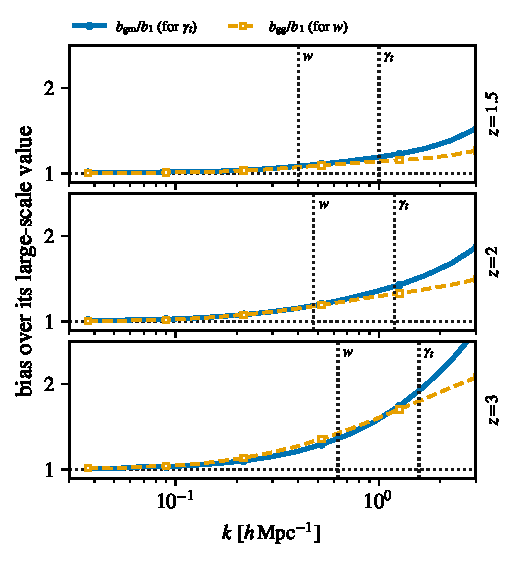
\includegraphics[width=0.55\textwidth]{plots/bias_k/bias_k.pdf}
\caption{Bias over its large-scale value $b_1$ for the FLAMINGO galaxies,
one panel per redshift: $\bgm/b_1$, which enters $\gamma_t$ (solid, filled
circles), and $\bgg/b_1$, which enters $w$ (dashed, open squares). The
horizontal dotted line is linear bias; the vertical dotted lines are
$k_{\max}$ of the $w$ and $\gamma_t$ cuts.}
\label{fig:bias_k}
\end{figure}

\textbf{The bias rises with $k$, faster at higher redshift}
(Figure~\ref{fig:bias_k}). At $z = 1.5$ both biases stay within 10\% of linear
below $k = 0.4\hMpc$; at $z = 3$ they are 15 to 20\% above linear already at
$k = 0.3\hMpc$. Because the cuts move to higher $k$ with redshift, the
departure at the cut grows steeply: \wA, \wB, \wC\% for $\bgg$ at the $w$
cut and \gA, \gB, \gC\% for $\bgm$ at the $\gamma_t$ cut. The high-redshift
lens bins, not the low ones, set how far linear bias can be used.

\textbf{$\bgm$ and $\bgg$ agree to $k \approx 0.5\hMpc$ at $z \le 2$.} The
$\gamma_t$ estimate made earlier from $\Pgg$ alone assumed $\Pgm = \bgg \Pm$,
that is $r = 1$. That holds to 1.5\% at $z = 1.5$ and 2 below
$k = 0.5\hMpc$, where $r = \rA$ and \rB\ at $k = 0.3\hMpc$. At $z = 3$
$\bgm$ is below $\bgg$ by up to 5\% between 0.2 and $0.6\hMpc$ ($r = \rC$
at 0.3). Beyond $k \approx 1\hMpc$, $\bgm$ grows faster than $\bgg$ at every
redshift.

\begin{figure}[!htbp]
\centering
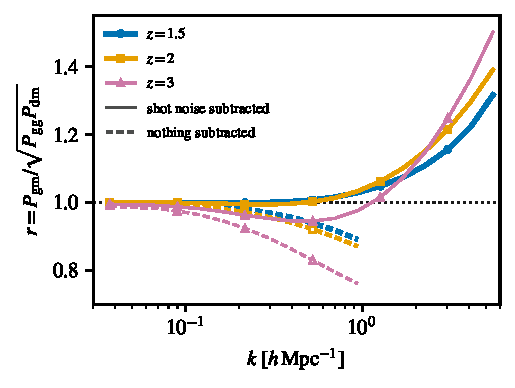
\includegraphics[width=0.55\textwidth]{plots/cross_r/cross_r.pdf}
\caption{Cross-correlation coefficient of galaxies and dark matter at
$z = 1.5$, 2, 3 (color, line width and marker). Solid with filled markers:
Poisson shot noise subtracted from $\Pgg$ and $\Pdm$, stitched over the
folds. Dashed with open markers: nothing subtracted, fold 1 only. The dotted
line is $r = 1$.}
\label{fig:cross_r}
\end{figure}

\textbf{Above $k \approx 1\hMpc$ the galaxy noise is not Poisson}
(Figure~\ref{fig:cross_r}). With the Poisson level subtracted, $r$ rises
above 1, to \rFiveLo\ to \rFiveHi\ at $k = 5\hMpc$, which a coefficient
cannot do. The subtraction removes more than the true noise: the galaxies are
sub-Poisson on small scales, as expected when each halo holds one central and
halos exclude each other. Without subtraction, $r$ is \rRawOneLo\ to
\rRawOneHi\ at $k = 1\hMpc$, a lower bound. So $\bgg$ and $r$ above
$1\hMpc$ carry a noise-model uncertainty; $\bgm$ does not, since the cross
spectrum has no shot noise of this kind. The noise matters at the $w$ cuts
too: the whole Poisson term is \ShotWA, \ShotWB\ and \ShotWC\% of $\bgg$ there
($z = 1.5$, 2, 3). At those scales the subtracted $r$ is still at or below 1,
as Poisson noise would give, but the noise level is not measured
independently.

\section{Checks}

\begin{itemize}
\item \textbf{Galaxy field.} $\Pgg$ from the new grids equals the IA
  pipeline's $P_{hh}$ bin for bin (ratio 1 to machine precision), and the
  galaxy counts equal those of the IA run.
\item \textbf{Folds.} $\bgm$ from fold 4 agrees with fold 1 to \FoldA, \FoldB\
  and \FoldC\% at $k = 0.3$ to $1\hMpc$ ($z = 1.5$, 2, 3). The absolute
  $\Pdm$ differs by 3\% between folds there (the grid window), and cancels in
  every ratio.
\item \textbf{Two biases.} $b_1$ from $\Pgm$ and from $\Pgg$ agree to 0.1\%
  at $z \le 2$ and 0.7\% at $z = 3$.
\item \textbf{Earlier estimate.} The earlier $b(k)$ from $P_{hh}$ and the
  SWIFT matter spectrum is reproduced: its shape
  $b(k)/b(0.04 < k < 0.1)$ at $k = 0.22$ to $0.94\hMpc$ agrees to \OldShape\%.
  Its large-scale value is \OldNorm\% higher, the grid window
  ($\Pdm^{\rm grid}/P_{\rm cdm}^{\rm SWIFT} = 1.01$ to 1.04 below
  $0.1\hMpc$) it did not divide out.
\end{itemize}

\section{Products and code}

\begin{sloppypar}
\begin{itemize}
\item Spectra: \texttt{flamingo/data/PS\_matter/} (\texttt{Pmm\_dm}, \texttt{Pgm},
  \texttt{Pgg} per snapshot and fold, rows $k$, $P$, $\sigma_P$, $N_{\rm modes}$;
  \texttt{matter\_cross\_sn<sn>.json} with $N$ and $V/N$).
\item Streaming and spectra: \texttt{flamingo/extraction/matter\_cross.py}, driven
  by \texttt{run\_matter\_cross.sh}.
\item Biases: \texttt{analysis/cut\_validation/galaxy\_bias/flamingo\_beta.py},
  writing \texttt{beta\_tables.npz} ($b_1$, $\bgm/b_1$, $(\bgg/b_1)^2$ on a
  common $k$ grid for all 13 snapshots; the snapshots without $\Pgm$ take $r$
  and the grid window from the nearest of $z = 1.5$, 2, 3).
\item Figures: \texttt{notes/flamingo\_pgm/plots/}, from
  \texttt{make\_figure\_data.py}.
\end{itemize}
\end{sloppypar}

\section{Open issues}

\begin{itemize}
\item \textbf{Tracer.} The galaxies are the IA shape sample. Roman's lens
  biases (1.24 to 2.52) are close to these at $z \le 2$, but their scale
  dependence is not measured here.
\item \textbf{Noise model.} $\bgg$ depends on the galaxy noise level, by up to
  \ShotWC\% at the $z = 3$ $w$ cut if it ranged from zero to Poisson; above
  $k \approx 1\hMpc$ it is sub-Poisson; the snapshots below $z = 1.5$ take
  $r$ from $z = 1.5$, including its values above 1 there.
\item \textbf{Errors.} The spectra come from one box and carry no error bars
  here; sample variance largely cancels in the ratios, but the $k < 0.03\hMpc$
  bins hold few modes.
\end{itemize}

\end{document}
